\documentclass[a4paper,10pt]{article}
\usepackage[T1]{fontenc}
\usepackage[utf8]{inputenc}
\usepackage{lmodern,textcomp}
\usepackage[margin=2.2cm]{geometry}
\usepackage{amsmath,amssymb,siunitx,booktabs,graphicx,tabularx,array,enumitem,xcolor,fancyhdr,float}
\usepackage[colorlinks=true,linkcolor=blue!50!black,urlcolor=blue!50!black]{hyperref}
\setlength{\parindent}{0pt}
\setlength{\parskip}{4pt}
\setlength{\headheight}{14pt}
\renewcommand{\arraystretch}{1.2}
\renewcommand{\tabularxcolumn}[1]{>{\raggedright\arraybackslash}p{#1}}
\setlist{nosep,leftmargin=*}
\newcommand{\file}[1]{\nolinkurl{#1}}
\sisetup{per-mode=symbol}
\pagestyle{fancy}\fancyhf{}
\fancyhead[L]{34870 Electroacoustics}
\fancyhead[R]{Lab C --- reference version (for checking)}
\fancyfoot[L]{Group 10}
\fancyfoot[R]{\thepage}
\graphicspath{{../figures/}{Lab C/figures/}{../ltspice/}{Lab C/ltspice/}}
\begin{document}
\begin{center}
{\Large\bfseries Lab C --- Microphone calibration}\\[5pt]
34870 Electroacoustics\\[4pt]
Group 10: Louis Andrianne, Sophie Kimura, Mads Rudolph\\[4pt]
Measured Tuesday 29 September 2026, building 354, room 026
\end{center}
\thispagestyle{fancy}

\fbox{\begin{minipage}{0.97\linewidth}\small
\textbf{Reference version.} This is a complete worked version of the lab, written to
check the group's own report against: the numbers, figures and conclusions below are
what the data give. The group's report is \file{LabC_report.tex}. All numbers come from
\file{Lab C/matlab/run_all.m}, which reads the untouched lab-PC files in
\file{Lab C/raw data/} and writes the figures in \file{Lab C/figures/}.
\end{minipage}}

\section{Purpose and set-up}
Two \textonehalf-inch condenser microphones, a B\&K 4133 (free field) and a B\&K 4134
(pressure field), were calibrated in two steps. First the absolute sensitivity was
measured at a single frequency with three GRAS 42AG sound calibrators. Then the frequency
response was measured with an electrostatic actuator, which drives the diaphragm with a
force that is practically independent of frequency. The response gives the shape, and the
calibrator gives the level. Resonance frequency and Q were read off the response and used
to set the backplate parameters of an LTspice model of the microphone.

All measurements used the NI USB-4431 card (\SI{96}{\kilo\hertz} sampling) and the
B\&K Nexus amplifier set to \SI{10}{\milli\volt\per\pascal} in and out
($G_{\mathrm{Nex}}=1$), \SI{0.1}{\hertz}/\SI{100}{\kilo\hertz} filters and
\SI{200}{\volt} polarisation. The capsules were only labelled ``Mic 1'' and ``Mic 2''
in the lab; which type is which follows from the measured responses
(Section~\ref{sec:which}). Serial numbers, calibrator certificates and room conditions
were not recorded; the room was at ordinary laboratory conditions.

\section{Part 1: the measurement system}
The generator output AO0 was connected to input AI0 and, through the Nexus, to input AI1.
The ratio
\begin{equation}
H_{21,\mathrm{ref}}(f)=\frac{V_{\mathrm{AI1}}(f)}{V_{\mathrm{AI0}}(f)}
\end{equation}
is the response of the measurement chain alone. It is divided out of every later
measurement: at \SI{250}{\hertz} and \SI{1}{\kilo\hertz} in Part 2, and at every
frequency in Part 3.

The multitone has six lines per octave from \SI{20}{\hertz} up to the requested
\SI{60}{\kilo\hertz}, but the card cannot measure anything above the Nyquist frequency
$f_s/2=\SI{48}{\kilo\hertz}$. The line at \SI{47.8}{\kilo\hertz} lies on the
anti-aliasing edge ($|H_{21,\mathrm{ref}}|=\SI{-5.8}{\decibel}$), and the line at
\SI{53.6}{\kilo\hertz} is a mirror image of \SI{42.4}{\kilo\hertz}. Both are left out, so
the usable band is \SI{20}{\hertz} to \SI{42.7}{\kilo\hertz} (68 lines).

\begin{figure}[H]\centering
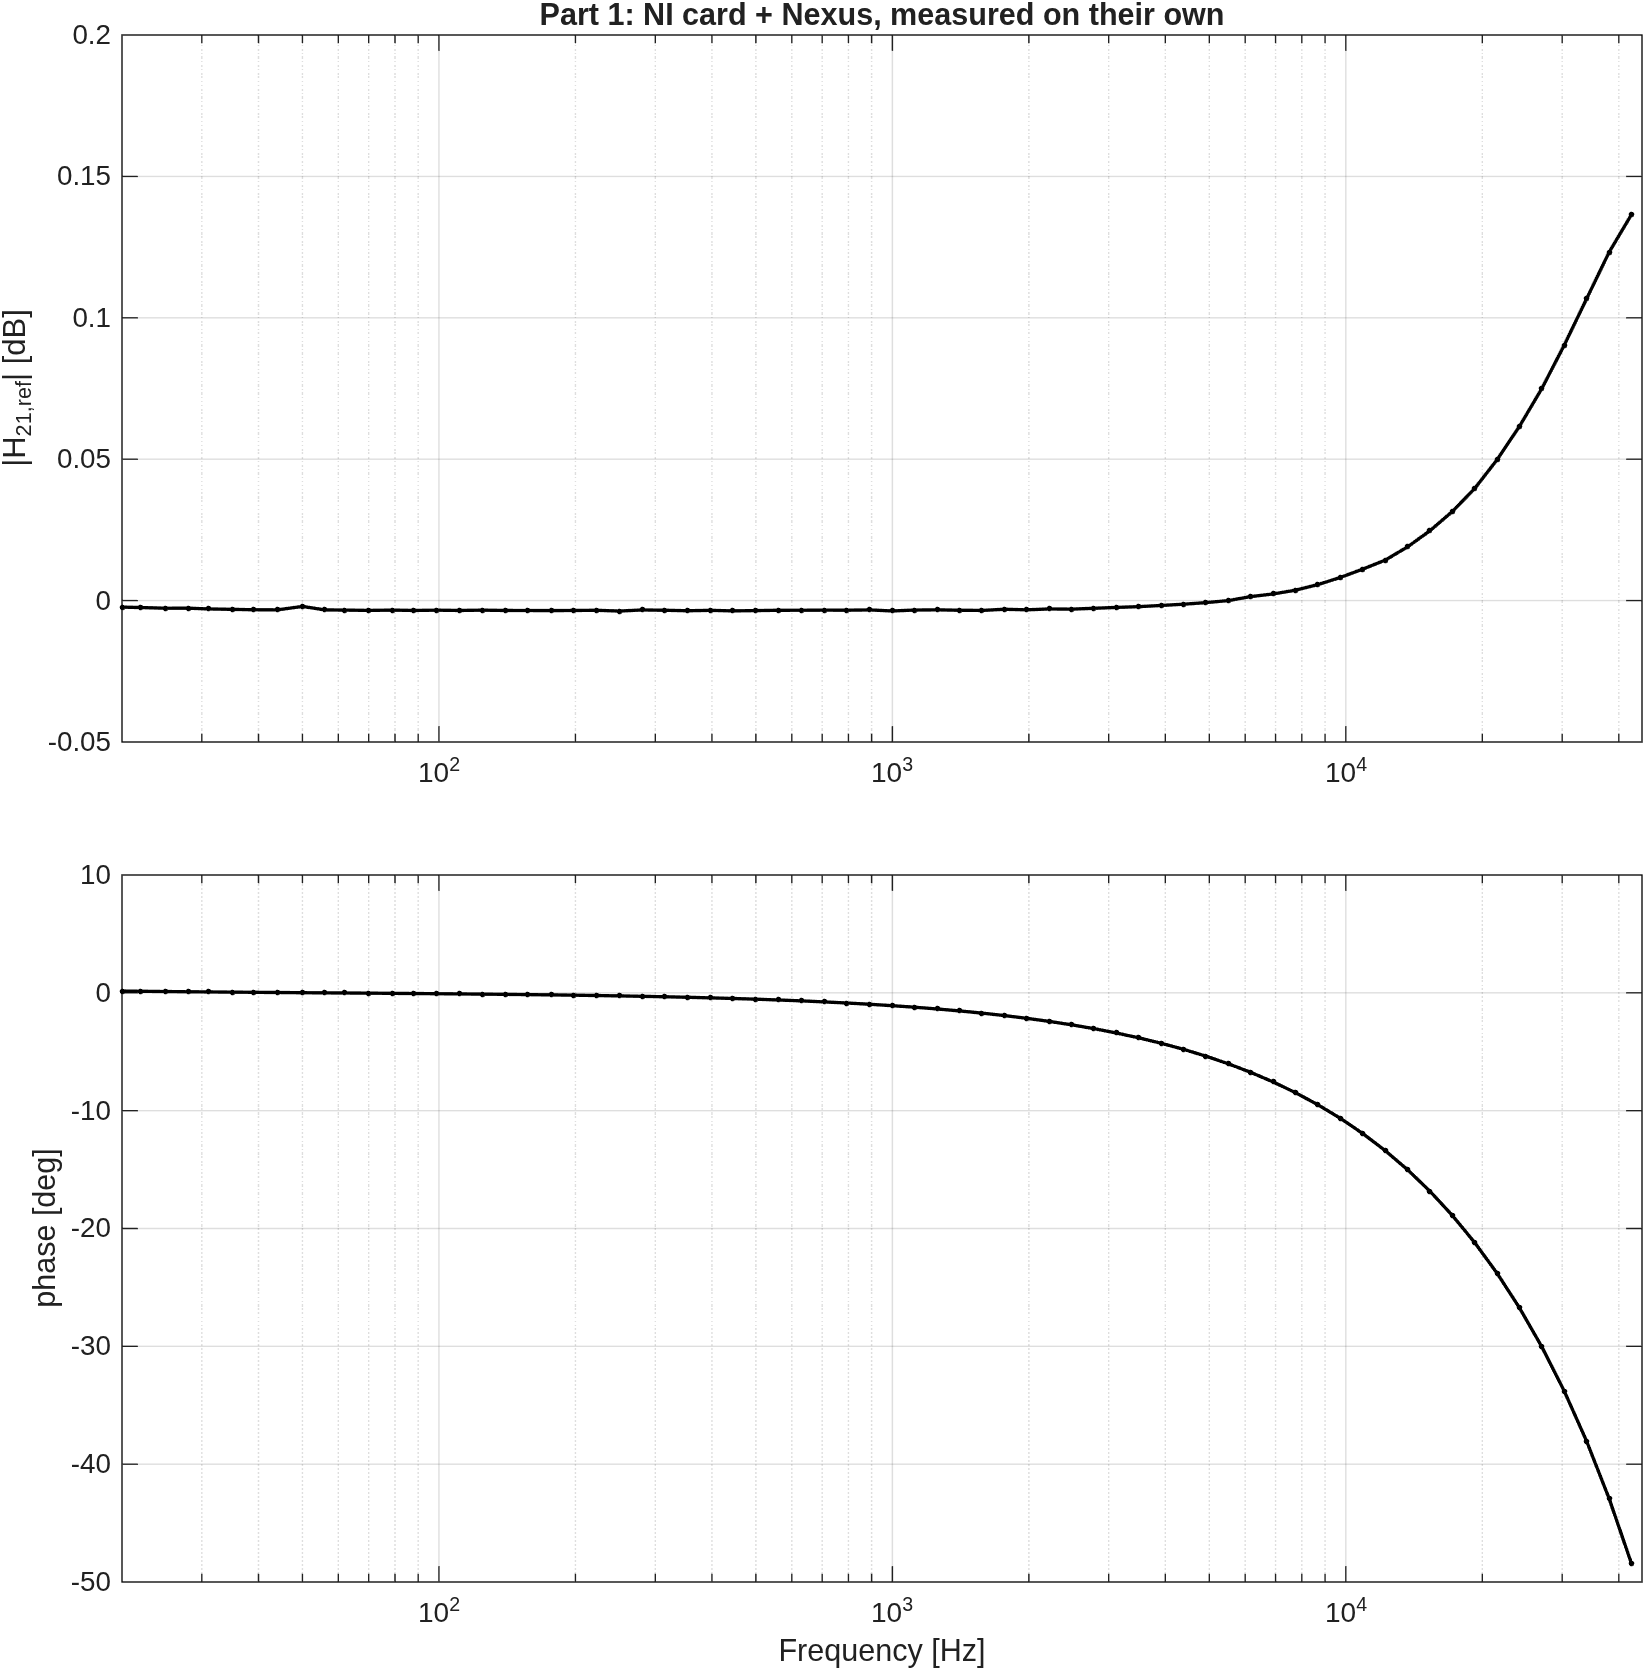
\includegraphics[width=0.8\linewidth]{labC_part1_system_reference.png}
\caption{System reference $H_{21,\mathrm{ref}}$. The magnitude stays within
\SI{0.15}{\decibel} of \SI{0}{\decibel}. The phase falls linearly to \SI{-48}{\degree}
at \SI{42}{\kilo\hertz}, which is a time delay of \SI{3.2}{\micro\second} between the
two input channels.}
\end{figure}

The phase is the reason the correction matters. Without it, the resonance frequency read
from the \SI{-90}{\degree} crossing would come out several kHz too low. At the two
calibration frequencies
\begin{equation}
|H_{21,\mathrm{ref}}(\SI{250}{\hertz})|=0.99957\;(\SI{-0.0037}{\decibel}),\qquad
|H_{21,\mathrm{ref}}(\SI{1}{\kilo\hertz})|=0.99958\;(\SI{-0.0037}{\decibel}).
\end{equation}

\section{Part 2: sensitivity at one frequency}
Each microphone was placed in each of the three calibrators, at \SI{250}{\hertz} and at
\SI{1}{\kilo\hertz}, with the frequency and level from each calibrator's label. The
course function \file{Calibrate} returns
\begin{equation}
M=\frac{v_{\mathrm{rms}}}{p_{\mathrm{rms}}\,G_{\mathrm{Nex}}},\qquad
p_{\mathrm{rms}}=\SI{20}{\micro\pascal}\cdot 10^{L_p/20},
\end{equation}
which is then divided by $|H_{21,\mathrm{ref}}|$ at the same frequency.

\paragraph{Correction of the stored values.} On the lab PC the \emph{dB values} of
$H_{21,\mathrm{ref}}$ ($-0.003607$ and $-0.003672$) were typed in instead of the linear
magnitudes (0.99957 and 0.99958). The stored sensitivities were therefore divided by
0.0036 instead of by 1, and they read about \SI{3}{\volt\per\pascal}. The correction is
\begin{equation}
M = M_{\mathrm{stored}}\cdot\frac{|\text{typed value}|}{|H_{21,\mathrm{ref}}|}.
\end{equation}
Table~\ref{tab:M} shows the corrected values.

\begin{table}[H]\centering
\caption{Corrected sensitivities in mV/Pa.}\label{tab:M}
\begin{tabular}{lcccc}\toprule
& \multicolumn{2}{c}{Mic 1 (4134)} & \multicolumn{2}{c}{Mic 2 (4133)}\\
\cmidrule(lr){2-3}\cmidrule(lr){4-5}
Calibrator & \SI{250}{\hertz} & \SI{1}{\kilo\hertz} & \SI{250}{\hertz} & \SI{1}{\kilo\hertz}\\\midrule
42AG no.\ 1 & 10.530 & 11.003 & 12.547 & 13.059\\
42AG no.\ 2 & 10.531 & 10.960 & 12.559 & 13.010\\
42AG no.\ 3 & 10.561 & 10.970 & 12.579 & 13.009\\\midrule
Mean & 10.541 & 10.978 & 12.562 & 13.026\\
Std.\ deviation & 0.017 & 0.023 & 0.016 & 0.028\\
Relative std.\ dev. & 0.16\,\% & 0.21\,\% & 0.13\,\% & 0.22\,\% \\
Level re \SI{1}{\volt\per\pascal} & \SI{-39.54}{\decibel} & \SI{-39.19}{\decibel} & \SI{-38.02}{\decibel} & \SI{-37.70}{\decibel}\\\bottomrule
\end{tabular}
\end{table}

\begin{figure}[H]\centering
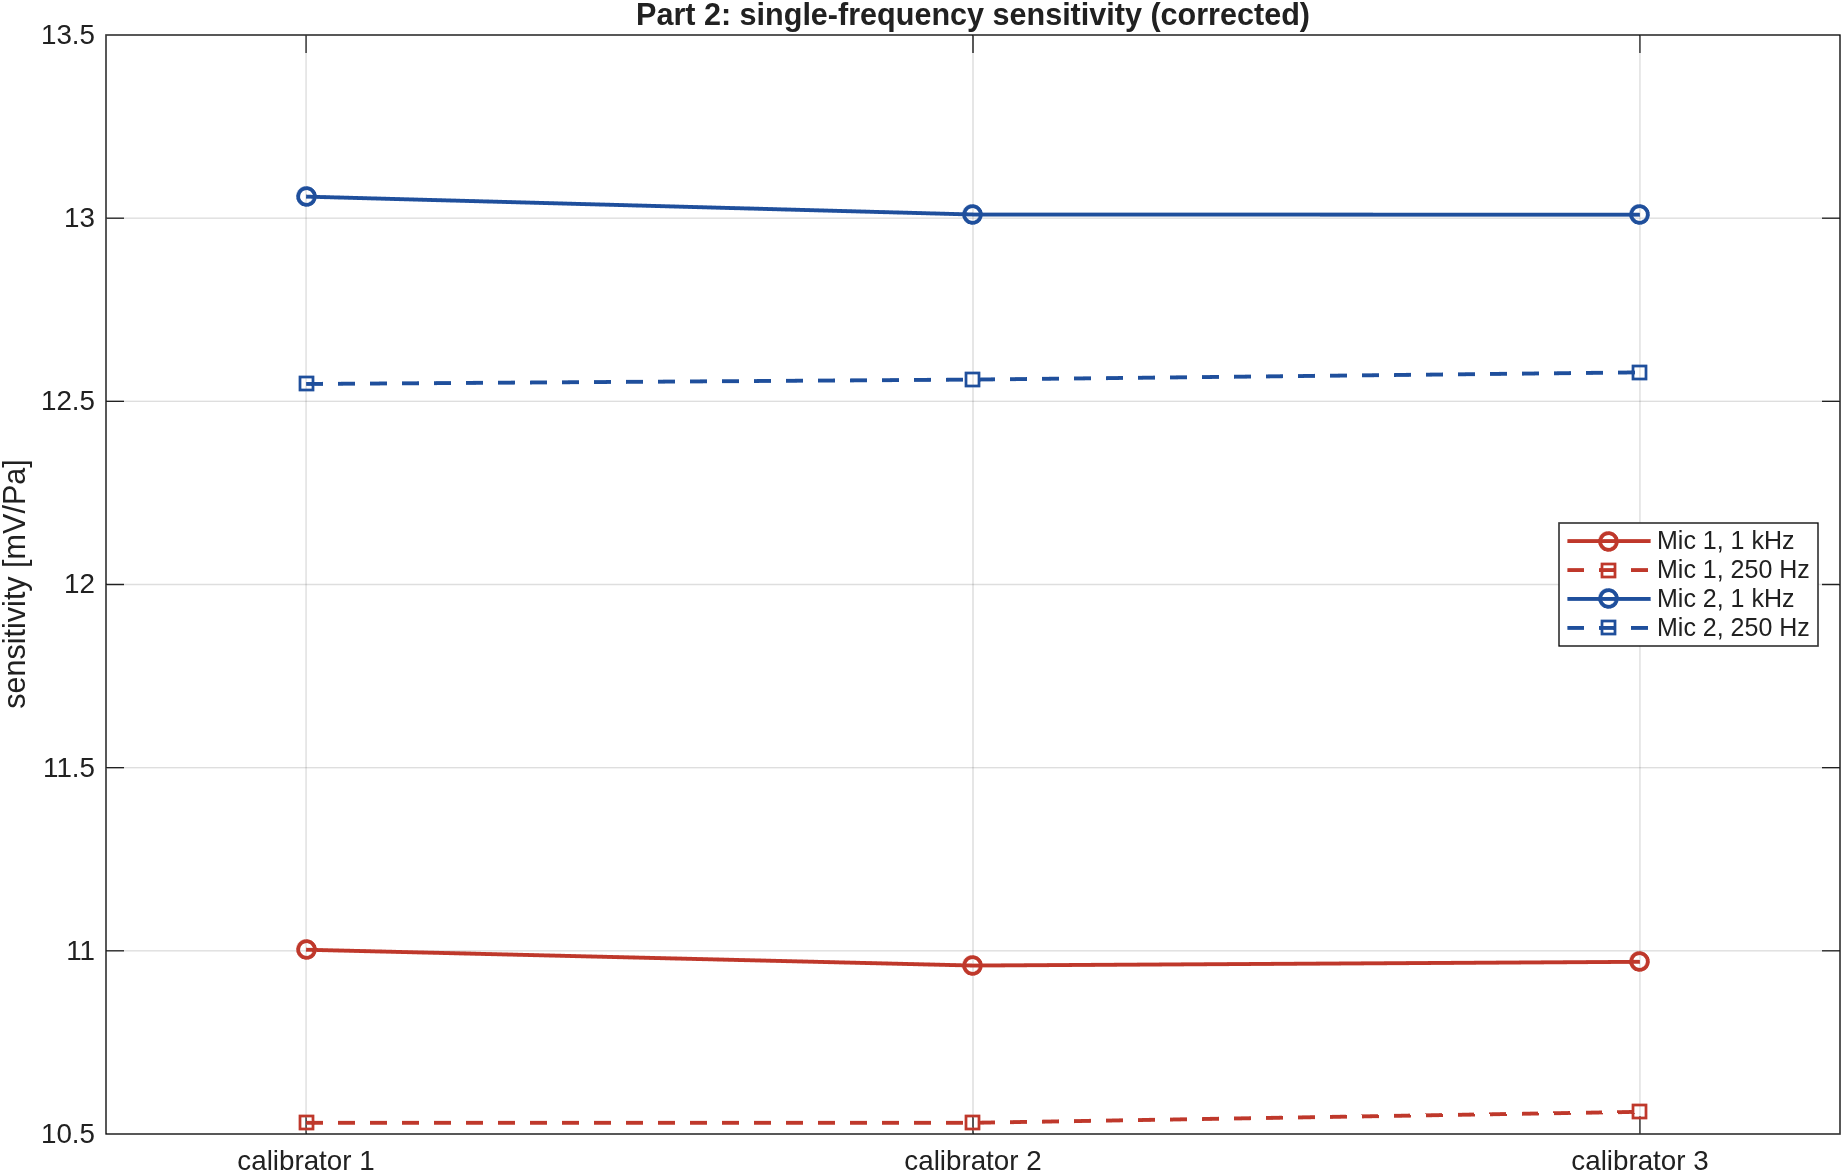
\includegraphics[width=0.62\linewidth]{labC_part2_sensitivity.png}
\caption{Sensitivity for each calibrator. The spread between calibrators is small, but
the \SI{250}{\hertz} results sit about \SI{0.35}{\decibel} below the \SI{1}{\kilo\hertz}
results for both microphones.}
\end{figure}

\paragraph{Repeatability, reproducibility and true value.}
\begin{itemize}
\item \textbf{Repeatability.} With the same microphone, the same method and three
calibrators, the results agree within 0.2\,\% (\SI{0.02}{\decibel}). The measurement
itself is very stable.
\item \textbf{Reproducibility.} Changing the method, here from \SI{1}{\kilo\hertz} to
\SI{250}{\hertz}, moves the result by \SI{-0.35}{\decibel} for Mic 1 and
\SI{-0.32}{\decibel} for Mic 2, about 4\,\%. Both microphones are flat within
\SI{0.1}{\decibel} between the two frequencies (Part 3), so the difference is not in the
microphones. It is the same for all three calibrators, so it is systematic. The most
likely cause is \file{Calibrate.m}: at \SI{250}{\hertz} it sums only six FFT bins ending
at the nominal frequency (the window was written for a \SI{251.2}{\hertz} pistonphone),
while at \SI{1}{\kilo\hertz} it sums seventeen bins around the tone. A tone slightly
above \SI{250}{\hertz} loses part of its power outside the window. The time signals were
not saved, so this is the most plausible explanation, not a proven one.
\item \textbf{True value.} The small spread shows that the method is repeatable, not that
it is right: a systematic error of 4\,\% is ten times larger than the spread and does
not show up in it. How close the result is to the true value depends on the traceable
uncertainty of the calibrators, not on the scatter of the readings.
\end{itemize}
The \SI{1}{\kilo\hertz} values are used from here on: Mic 1 $M=\SI{10.98}{\milli\volt\per\pascal}$,
Mic 2 $M=\SI{13.03}{\milli\volt\per\pascal}$.

\paragraph{Uncertainty budget (\SI{1}{\kilo\hertz}, Mic 1).}
The certificates were not recorded. The calibrator figure below is therefore the class-1
tolerance of IEC~60942, taken as an assumed value, not a certificate value.

\begin{table}[H]\centering\small
\begin{tabularx}{\linewidth}{@{}lXcc@{}}\toprule
Contribution & Basis & $u$ [dB] & $u$ [\%]\\\midrule
Calibrator level & $\pm\SI{0.2}{\decibel}$ tolerance (assumed), rectangular: $0.2/\sqrt3$ & 0.115 & 1.3\\
Repeatability of the mean & $s/\sqrt{3}=0.023/\sqrt3$ mV/Pa & 0.011 & 0.12\\
System correction $|H_{21,\mathrm{ref}}|$ & measured, varies by $<\SI{0.001}{\decibel}$ between lines & 0.001 & 0.01\\
Static pressure / temperature & not measured, ordinary room (assumed $\pm\SI{0.05}{\decibel}$, rectangular) & 0.029 & 0.33\\\midrule
Combined $u_c$ & root sum of squares & 0.12 & 1.4\\
Expanded $U$ ($k=2$, about 95\,\%) & & 0.24 & 2.8\\\bottomrule
\end{tabularx}
\end{table}
Result: Mic 1 (4134) $M = \SI{10.98}{\milli\volt\per\pascal} \pm \SI{0.31}{\milli\volt\per\pascal}$,
Mic 2 (4133) $M = \SI{13.03}{\milli\volt\per\pascal} \pm \SI{0.36}{\milli\volt\per\pascal}$ ($k=2$).
The budget is dominated by the calibrator. The \SI{0.35}{\decibel} method offset at
\SI{250}{\hertz} is larger than the whole budget. That is why a known systematic effect
has to be removed or explained, not simply added to the spread.

\section{Part 3: frequency response with the actuator}
\subsection{Noise floor}
With the actuator amplifier switched off, the microphone output was recorded with 4 and
with 64 averages (Mic 2 only). The noise is shown in the same normalisation as the
response (microphone channel over drive channel).

\begin{figure}[H]\centering
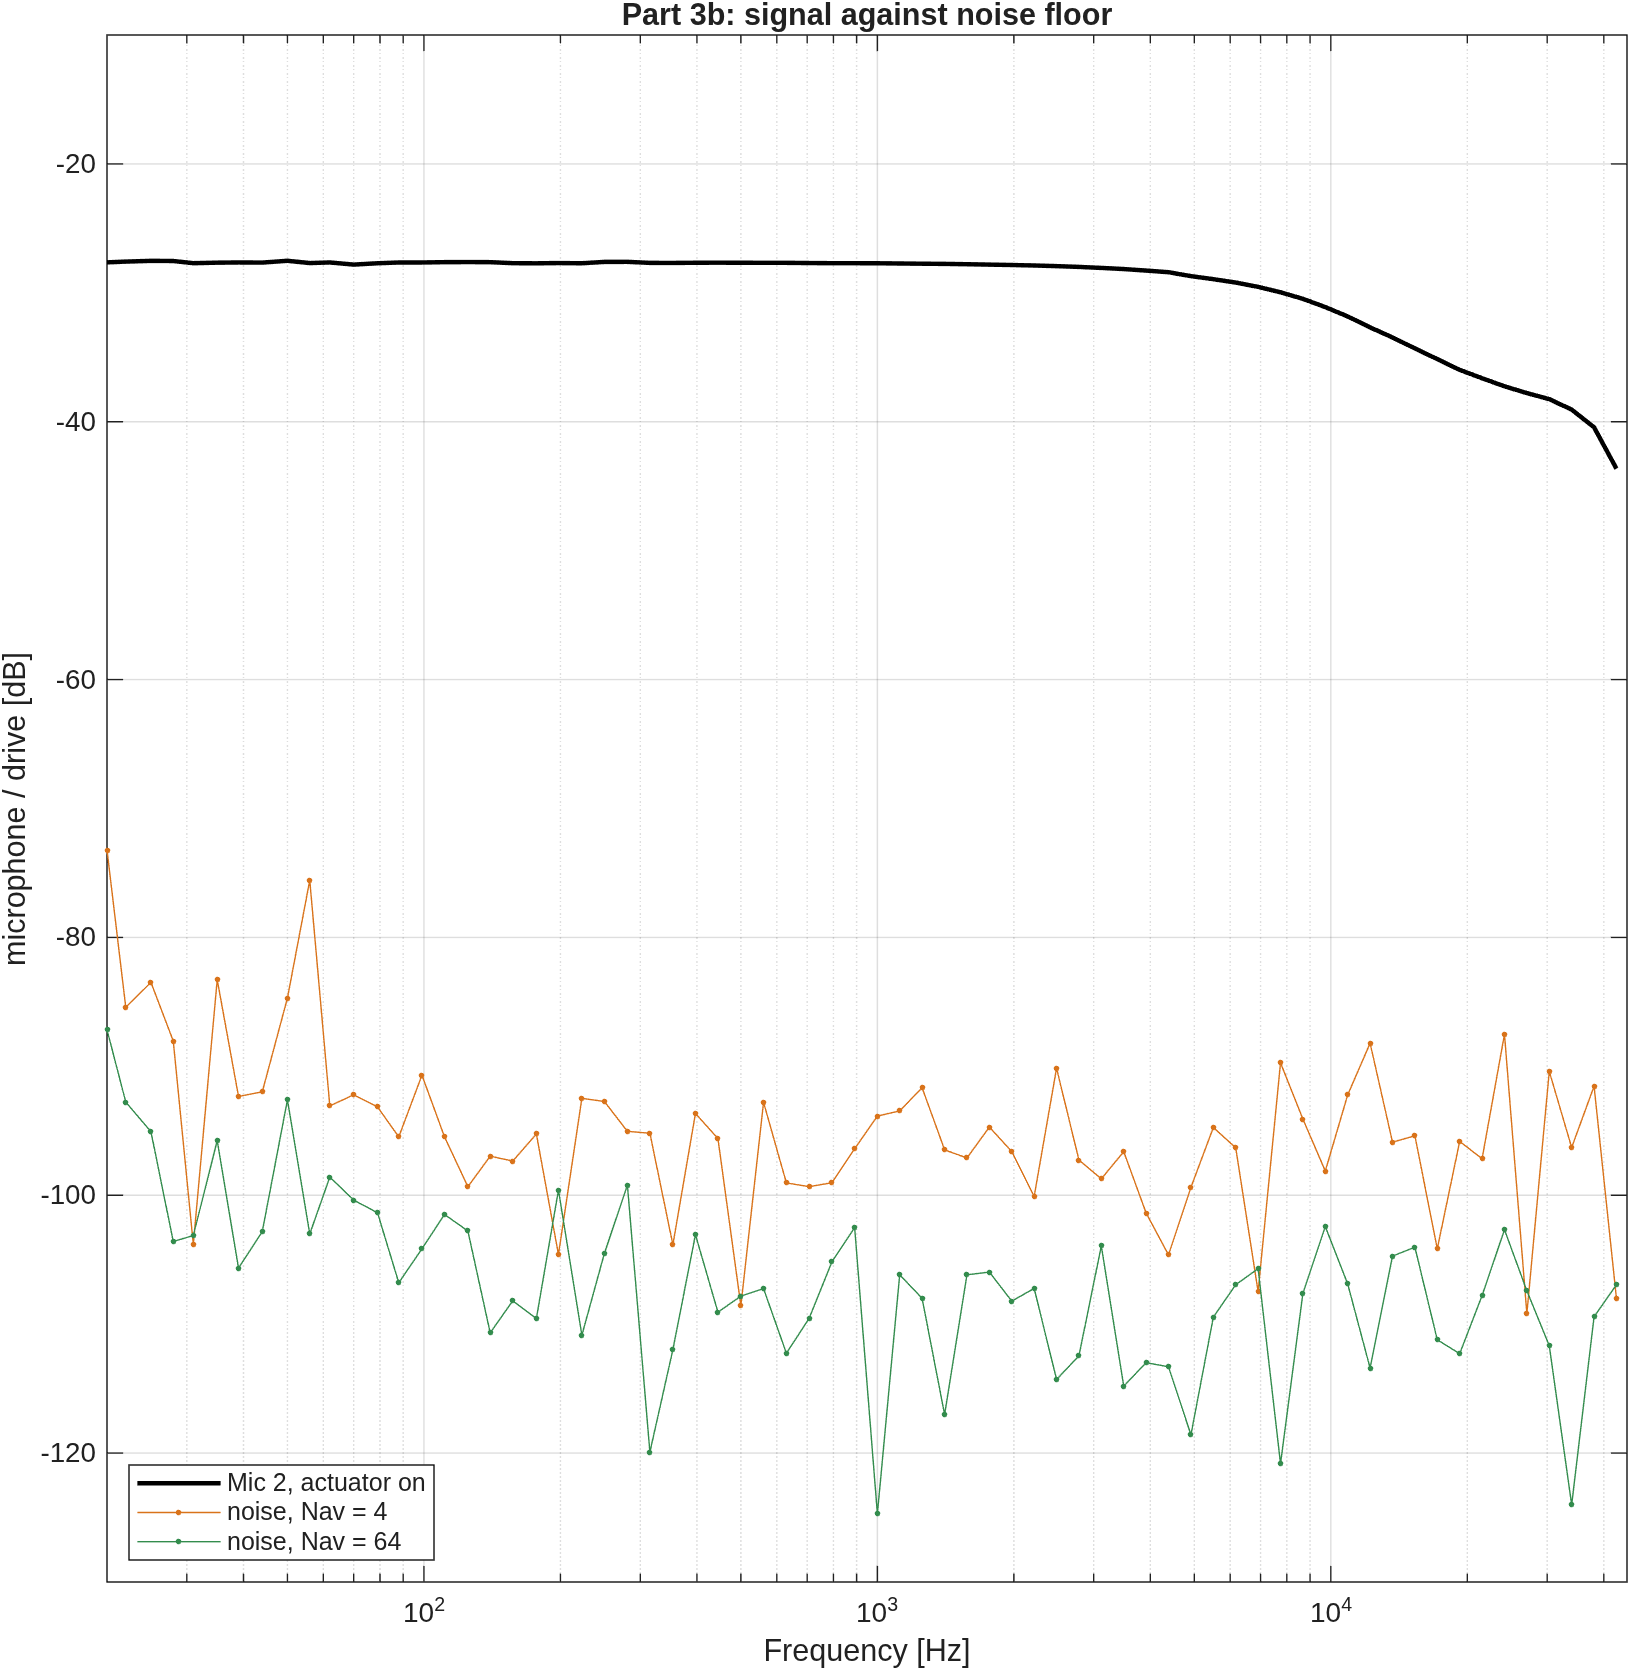
\includegraphics[width=0.72\linewidth]{labC_part3_noise_floor.png}
\caption{Actuator response of Mic 2 against the noise floor.}
\end{figure}

The signal is 60 to \SI{90}{\decibel} above the noise over most of the band. The worst
case is \SI{46}{\decibel} (4 averages) and \SI{60}{\decibel} (64 averages), both at
\SI{20}{\hertz}, where the room noise is highest. Going from 4 to 64 averages lowered the
noise by a median of \SI{11.6}{\decibel}. Averaging uncorrelated noise predicts
$10\log_{10}16=\SI{12.0}{\decibel}$, so the noise is random and not a disturbance locked
to the signal. The noise has no influence on the responses.

\subsection{Responses and identification of the microphones}\label{sec:which}
The measurement system is removed by
\begin{equation}
H_{pv}(f)=\frac{H_{21}(f)}{H_{21,\mathrm{ref}}(f)},
\end{equation}
and each curve is scaled to its \SI{1}{\kilo\hertz} sensitivity,
\begin{equation}
M(f)=M(\SI{1}{\kilo\hertz})\,\frac{H_{pv}(f)}{|H_{pv}(\SI{1}{\kilo\hertz})|}.
\end{equation}
The calibrator is a small closed coupler, so like the actuator it gives the \emph{pressure}
sensitivity. At \SI{1}{\kilo\hertz} the free-field correction of a \textonehalf-inch
microphone is practically zero, so the \SI{1}{\kilo\hertz} value is the right one for
both microphones. It is also the calibration without the systematic offset.

\begin{figure}[H]\centering
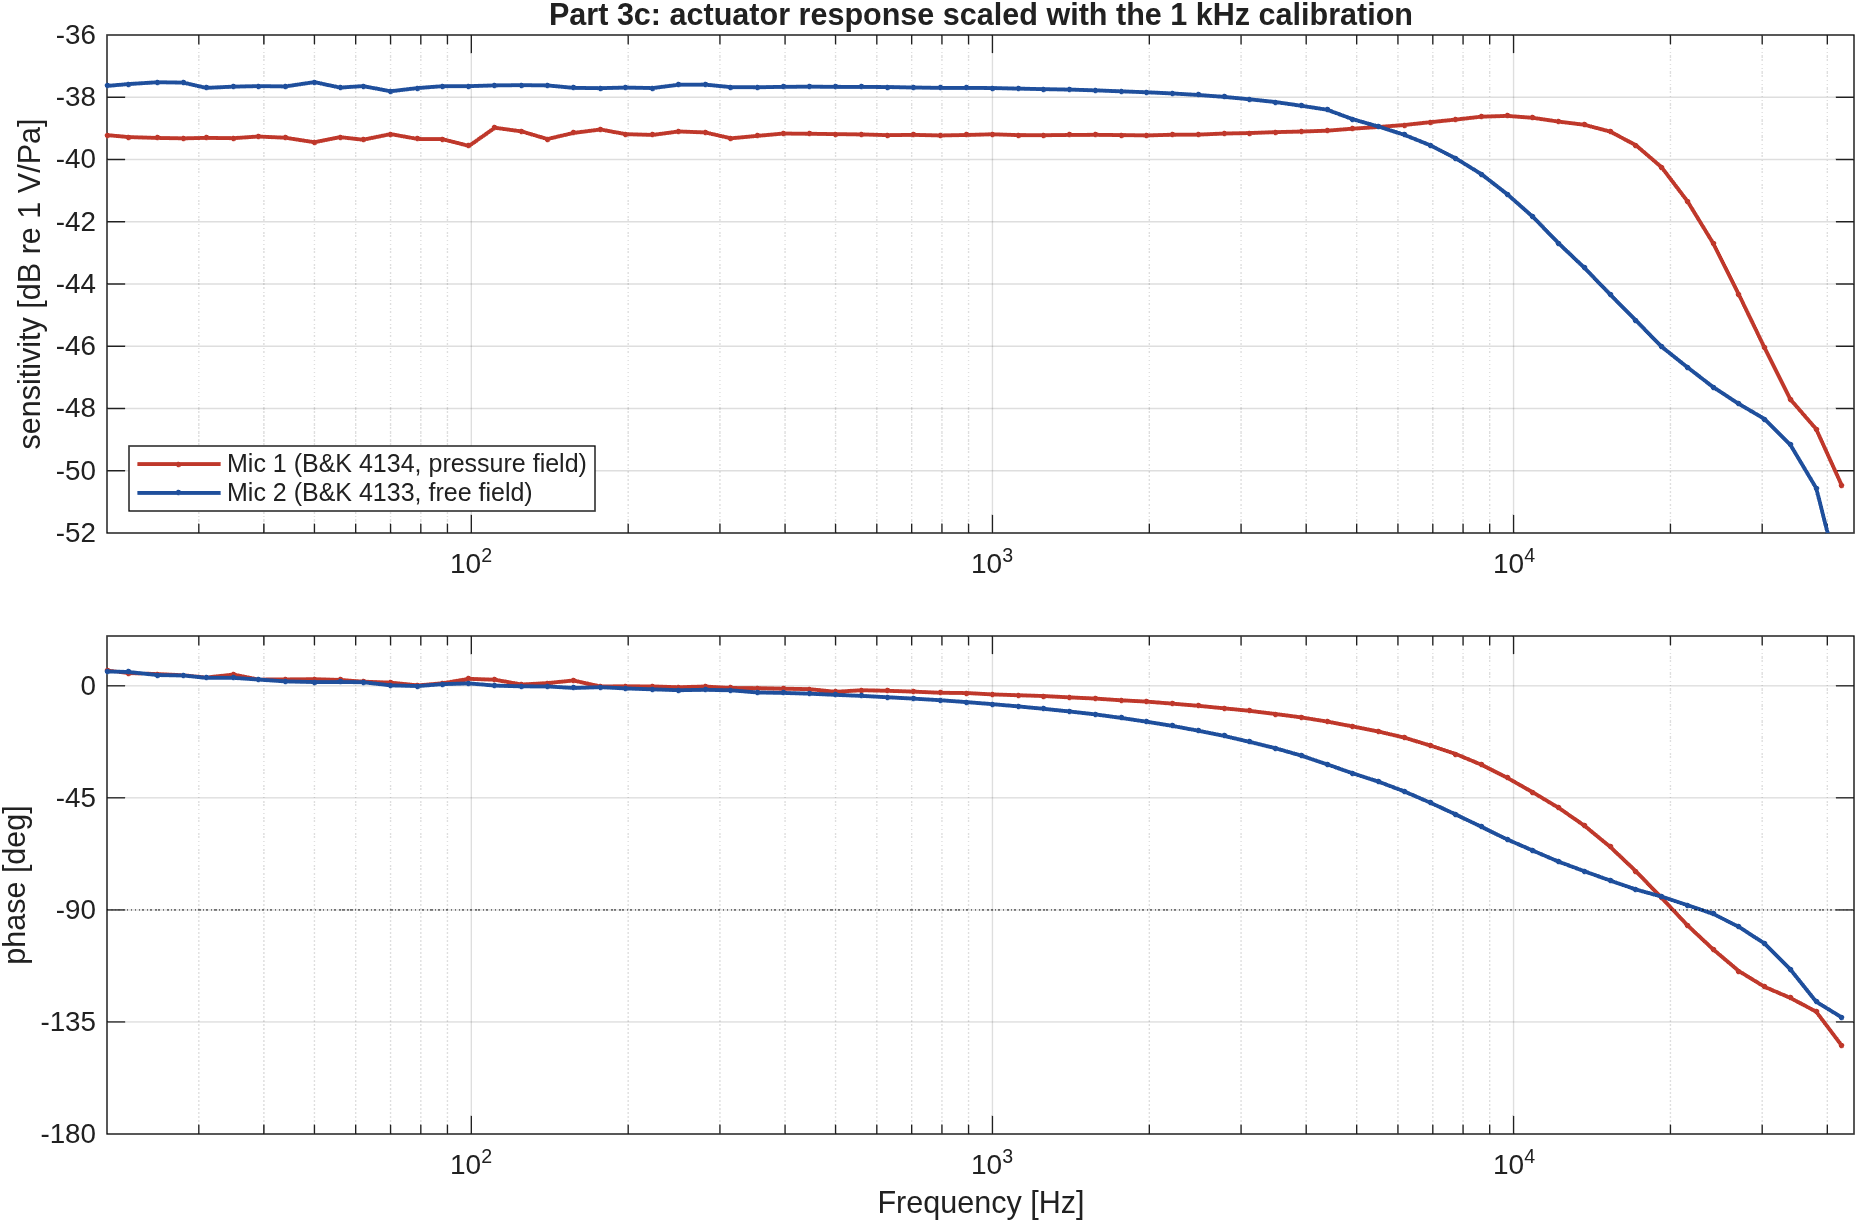
\includegraphics[width=0.85\linewidth]{labC_part3_responses.png}
\caption{Actuator responses scaled with the \SI{1}{\kilo\hertz} calibration.}
\end{figure}

\begin{itemize}
\item \textbf{Mic 1} is flat, rises by \SI{0.55}{\decibel} around \SI{10}{\kilo\hertz}
and is \SI{1.4}{\decibel} down at \SI{20}{\kilo\hertz}. A flat response to a uniform
pressure is the design goal of a \emph{pressure-field} microphone, so Mic 1 is the
\textbf{B\&K 4134}.
\item \textbf{Mic 2} is \SI{3.6}{\decibel} down at \SI{10}{\kilo\hertz} and
\SI{8.6}{\decibel} down at \SI{20}{\kilo\hertz}. The diaphragm is deliberately
over-damped: in a free field, diffraction around the microphone raises the pressure on
the diaphragm at high frequencies (the same scattering measured on the cylinder in
Lab~B). The falling pressure response cancels that rise. Mic 2 is therefore the
\emph{free-field} microphone, the \textbf{B\&K 4133}.
\end{itemize}

\section{Resonance frequency and Q}
Following the course slides (lectures 4 and 6), below resonance the diaphragm is
stiffness controlled (phase \SI{0}{\degree}), above it mass controlled
(\SI{-180}{\degree}). The resonance is where
\begin{equation}
\angle H_{pv}(f_s) = \SI{-90}{\degree},\qquad
Q=\frac{|H_{pv}(f_s)|}{|H_{pv}(f\ll f_s)|},
\end{equation}
with log-frequency interpolation between the measured lines and the low-frequency level
taken as the mean over \SI{100}{\hertz}--\SI{500}{\hertz}. As a cross-check, the
second-order function
\begin{equation}
H(f)=\frac{G}{1-(f/f_s)^2+\mathrm{j}(f/f_s)/Q}
\end{equation}
was fitted by least squares to the complex $H_{pv}$ from \SI{100}{\hertz} to
\SI{42.7}{\kilo\hertz}.

\begin{table}[H]\centering
\begin{tabular}{lcccc}\toprule
& \multicolumn{2}{c}{Slide procedure} & \multicolumn{2}{c}{Least-squares fit}\\
\cmidrule(lr){2-3}\cmidrule(lr){4-5}
Microphone & $f_s$ [kHz] & $Q$ & $f_s$ [kHz] & $Q$\\\midrule
Mic 1, 4134 (pressure) & 20.22 & 0.835 & 20.78 & 0.813\\
Mic 2, 4133 (free field) & 22.93 & 0.340 & 21.08 & 0.388\\\bottomrule
\end{tabular}
\end{table}

For the 4134 the two methods agree within 3\,\%. For the 4133 they differ by 9\,\% in
$f_s$ and 14\,\% in $Q$. The reason is visible in the phase: it falls slowly between
about 12 and \SI{25}{\kilo\hertz} and then faster than a single mass--spring--damper
would. The strong damping of a free-field capsule comes
from the air film between the diaphragm and a slotted, perforated backplate, and that
damping depends on frequency. A one-point reading and a whole-curve fit then weight
different parts of the curve.

\section{Model of the condenser microphone}
\subsection{Parameters}
The brief gives the same data for both capsules: gap $x_0=\SI{20.77}{\micro\metre}$,
polarisation $E=\SI{200}{\volt}$, effective diameter \SI{8.95}{\milli\metre}, diaphragm
mass $M_{MD}=\SI{1.5}{\milli\gram}$, compliance $C_{MD}=\SI{0.02}{\milli\metre\per\newton}$,
no diaphragm damping, back volume $V_B=\SI{126.4}{\milli\metre\cubed}$. With
$\rho=\SI{1.18}{\kilo\gram\per\metre\cubed}$ and $c=\SI{344}{\metre\per\second}$:
\begin{align}
S_D&=\pi a^2=\SI{6.291e-5}{\metre\squared}, &
C_{AB}&=\frac{V_B}{\rho c^2}=\SI{9.05e-13}{\metre\tothe{5}\per\newton}, &
M_{A1}&=\frac{0.6133\rho}{\pi a}=\SI{51.5}{\kilo\gram\per\metre\tothe{4}},
\end{align}
\begin{equation}
\frac{1}{C_{MT}}=\frac{1}{C_{MD}}+\frac{S_D^2}{C_{AB}}\;\Rightarrow\;C_{MT}=\SI{18.4}{\micro\metre\per\newton},
\end{equation}
\begin{equation}
C_{E0}=\frac{\varepsilon_0 S_D}{x_0}=\SI{26.8}{\pico\farad},\qquad
M_{\mathrm{model}}=\frac{E\,C_{MT}S_D}{x_0}=\SI{11.14}{\milli\volt\per\pascal}.
\end{equation}
The back volume stiffens the diaphragm by about 9\,\%. The measured $f_s$ fixes the
total moving mass and $Q$ fixes the resistance, so the backplate mass and resistance
follow:
\begin{equation}
M_{MT}=\frac{1}{(2\pi f_s)^2C_{MT}},\qquad
M_{AS}=\frac{M_{MT}-M_{MD}}{S_D^2}-M_{A1},\qquad
R_{AS}=\frac{1}{Q\,S_D^2}\sqrt{\frac{M_{MT}}{C_{MT}}}.
\end{equation}

\begin{table}[H]\centering
\begin{tabular}{lcccc}\toprule
Microphone & $f_s$ [Hz] & $Q$ & $M_{AS}$ [\si{\kilo\gram\per\metre\tothe{4}}] & $R_{AS}$ [\si{\pascal\second\per\metre\cubed}]\\\midrule
4134 (Mic 1) & 20\,221 & 0.835 & 420.5 & \num{1.29e8}\\
4133 (Mic 2) & 22\,930 & 0.340 & 231.4 & \num{2.80e8}\\\bottomrule
\end{tabular}
\end{table}
Both values are positive and physically sensible. The diaphragm alone would resonate at
\SI{28.4}{\kilo\hertz}; the air moved through the backplate holes lowers this to the
measured values. The free-field capsule has about twice the backplate resistance, which
is the damping that gives it its low $Q$.

\subsection{LTspice circuit}
The circuit uses three domains: acoustic in the impedance analogy, mechanical in the
mobility analogy, and electrical. The actuator is a \SI{1}{\pascal} source applied
directly to the diaphragm. There is no $G_{pb}$ generator for the diffraction function
$T(s)$, because the actuator does not create a sound field. Only $f_s$ and $Q$ are typed
in; LTspice computes $M_{AS}$ and $R_{AS}$ from them with the formulas above.

\begin{figure}[H]\centering
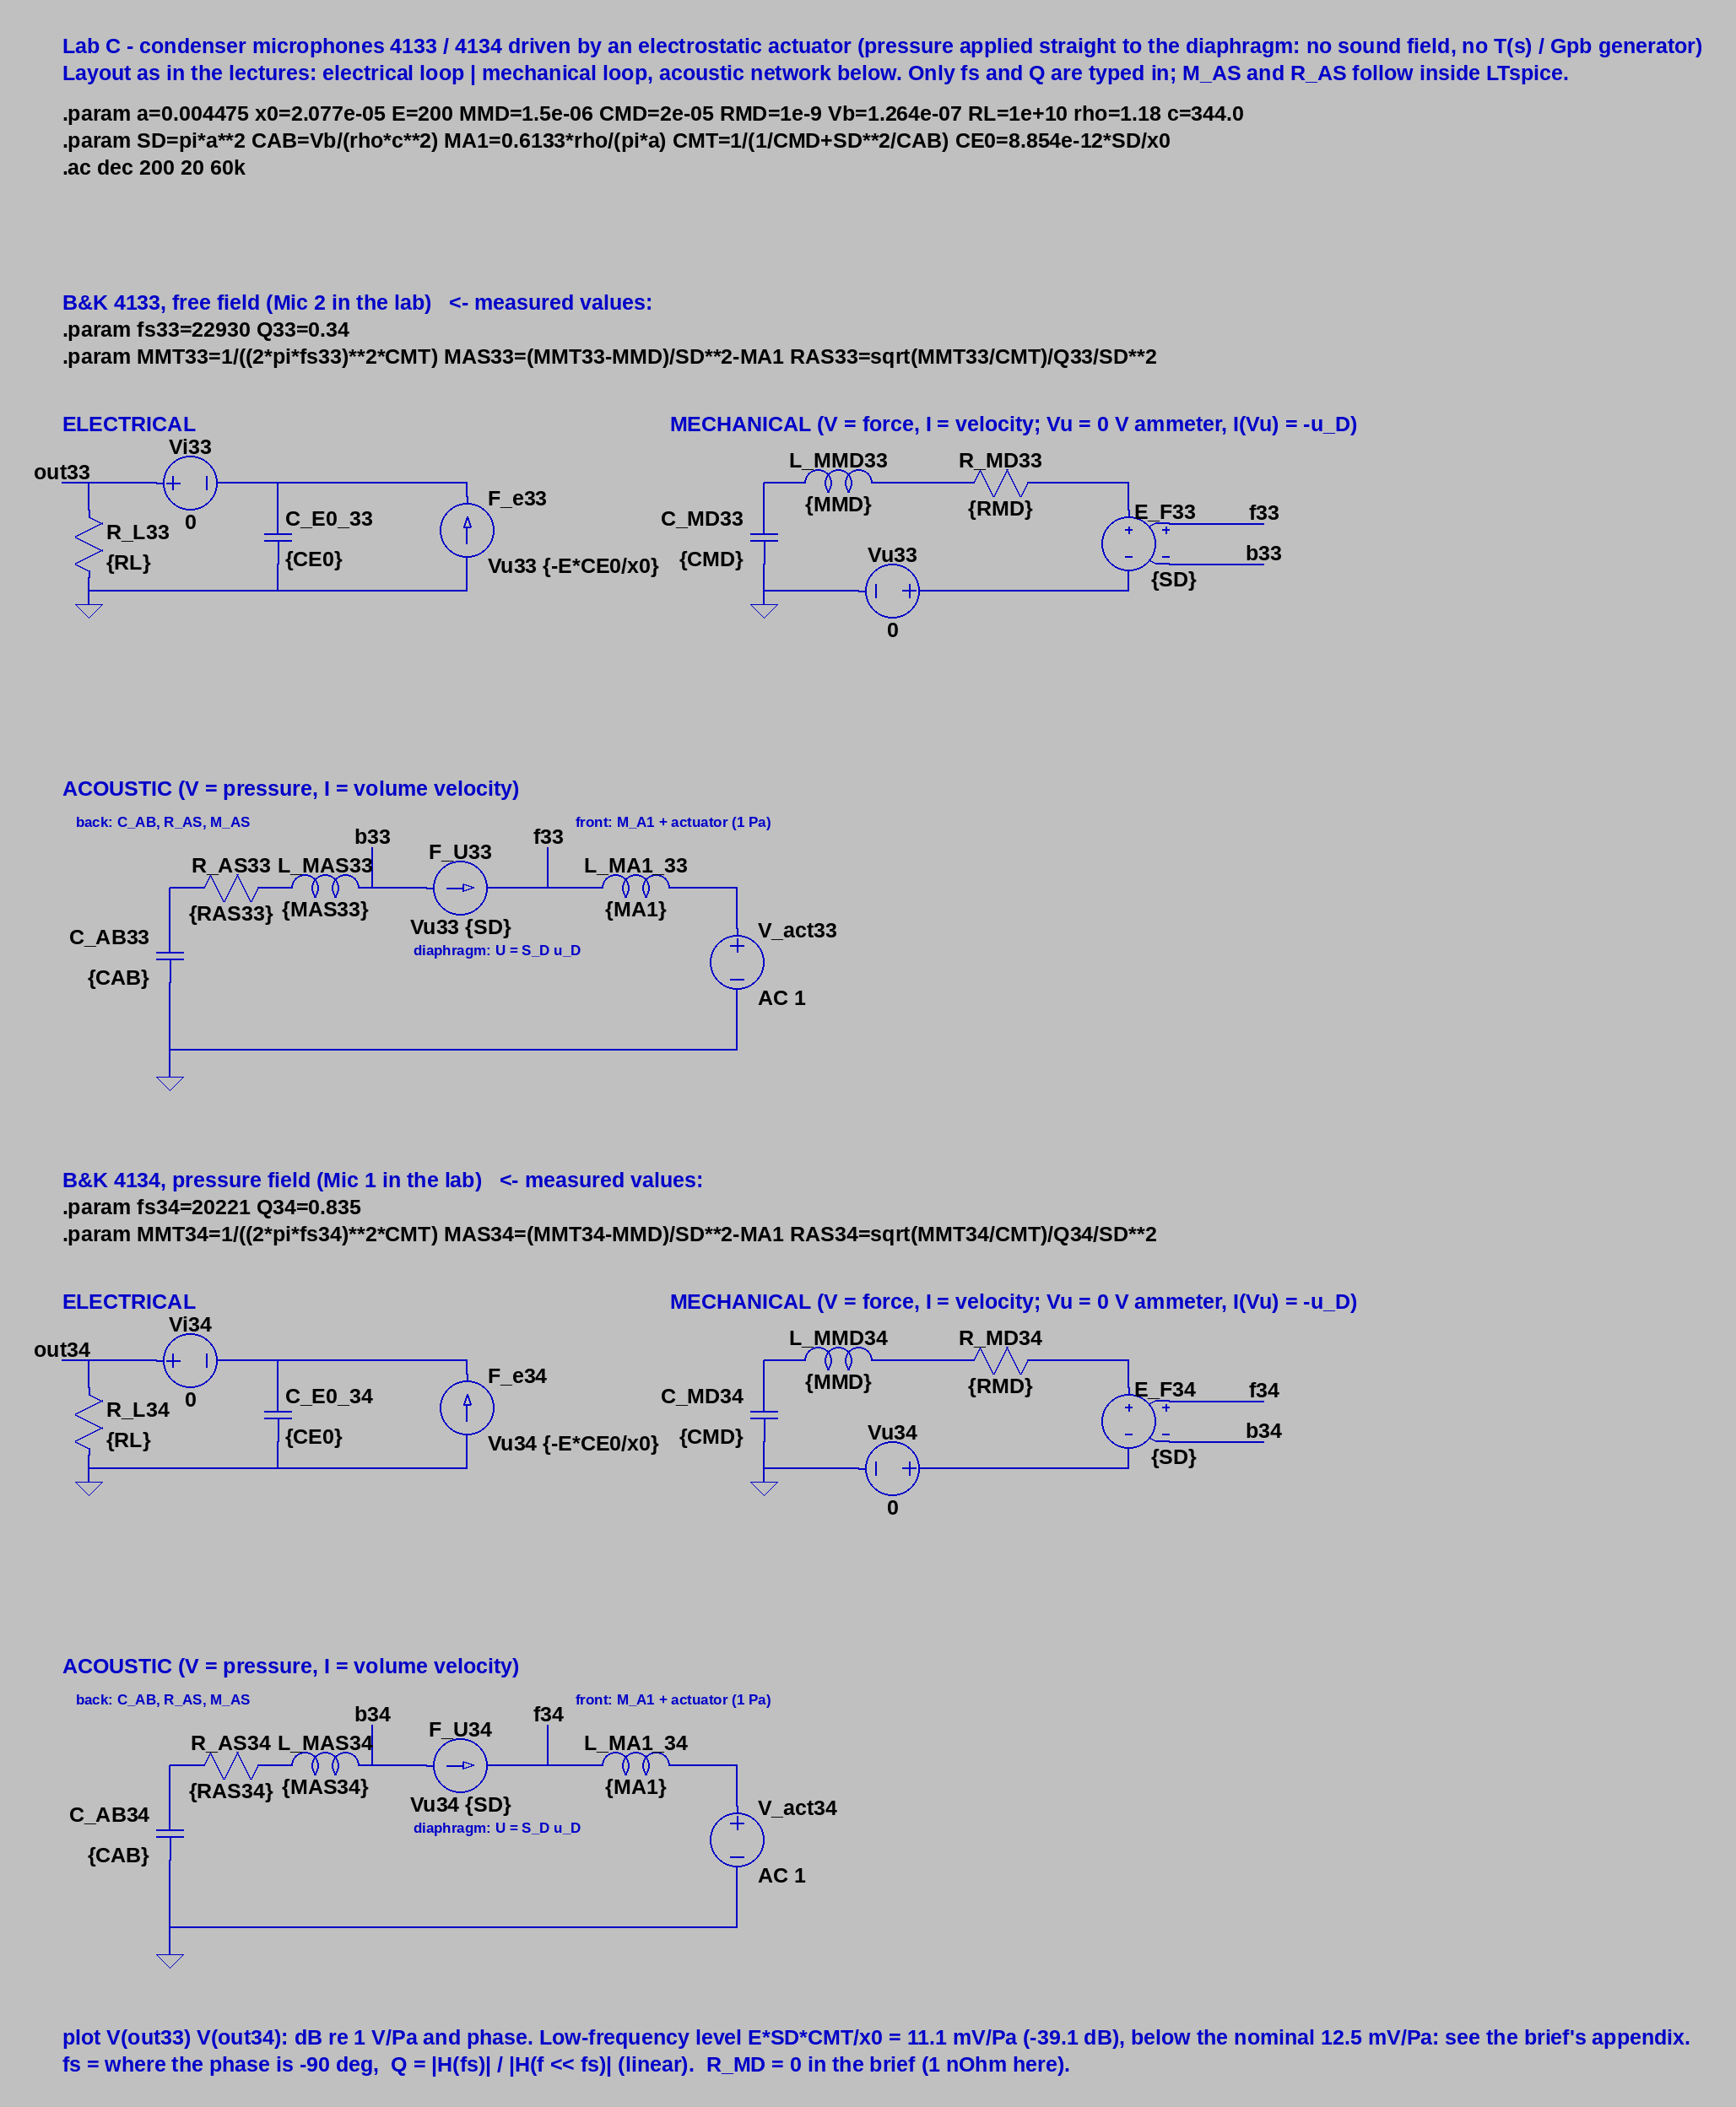
\includegraphics[width=\linewidth]{LabC_CondenserMics_preview.png}
\caption{LTspice schematic \file{LabC_CondenserMics.asc} (rendered preview).}
\end{figure}

\subsection{Model against measurement}
\begin{figure}[H]\centering
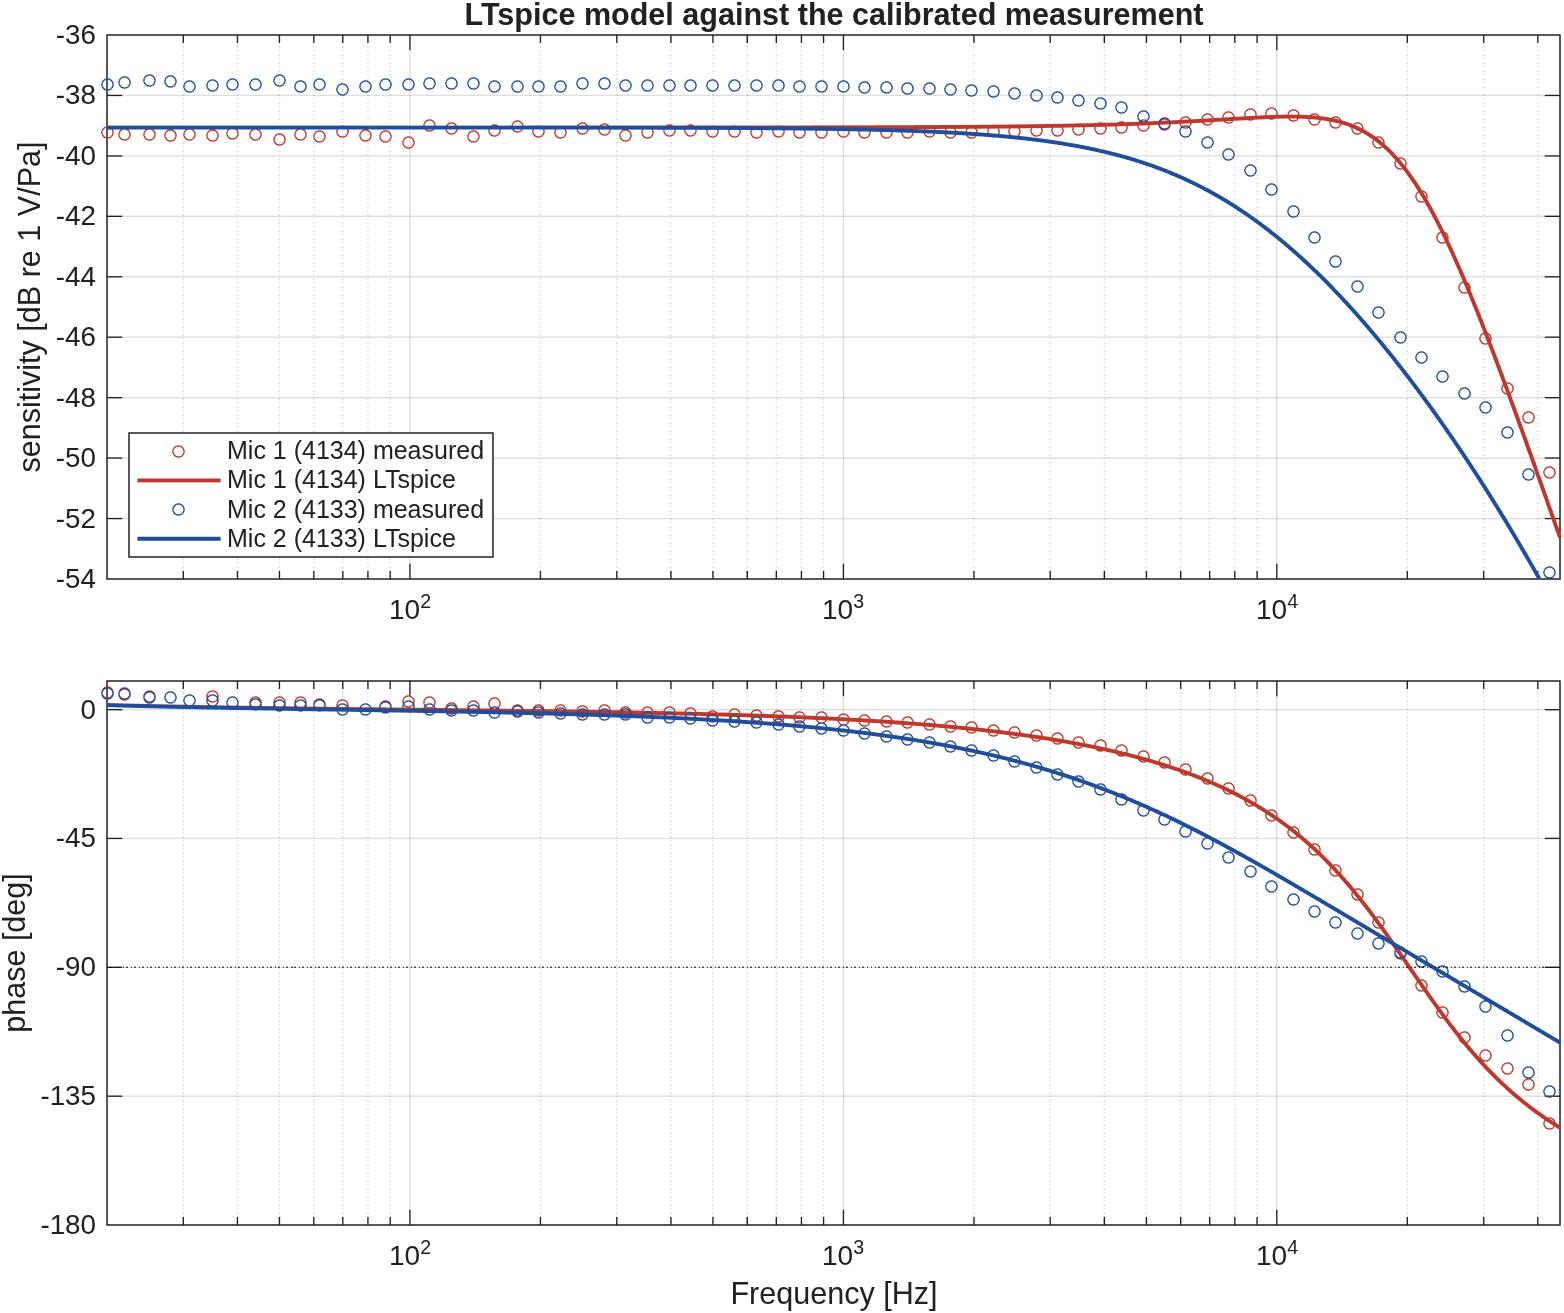
\includegraphics[width=0.85\linewidth]{labC_ltspice_vs_measurement.png}
\caption{LTspice output (lines) against the calibrated measurement (circles), in
absolute sensitivity. The LTspice source is entered with \SI{180}{\degree} phase, so no
extra phase shift is needed.}
\end{figure}

\begin{figure}[H]\centering
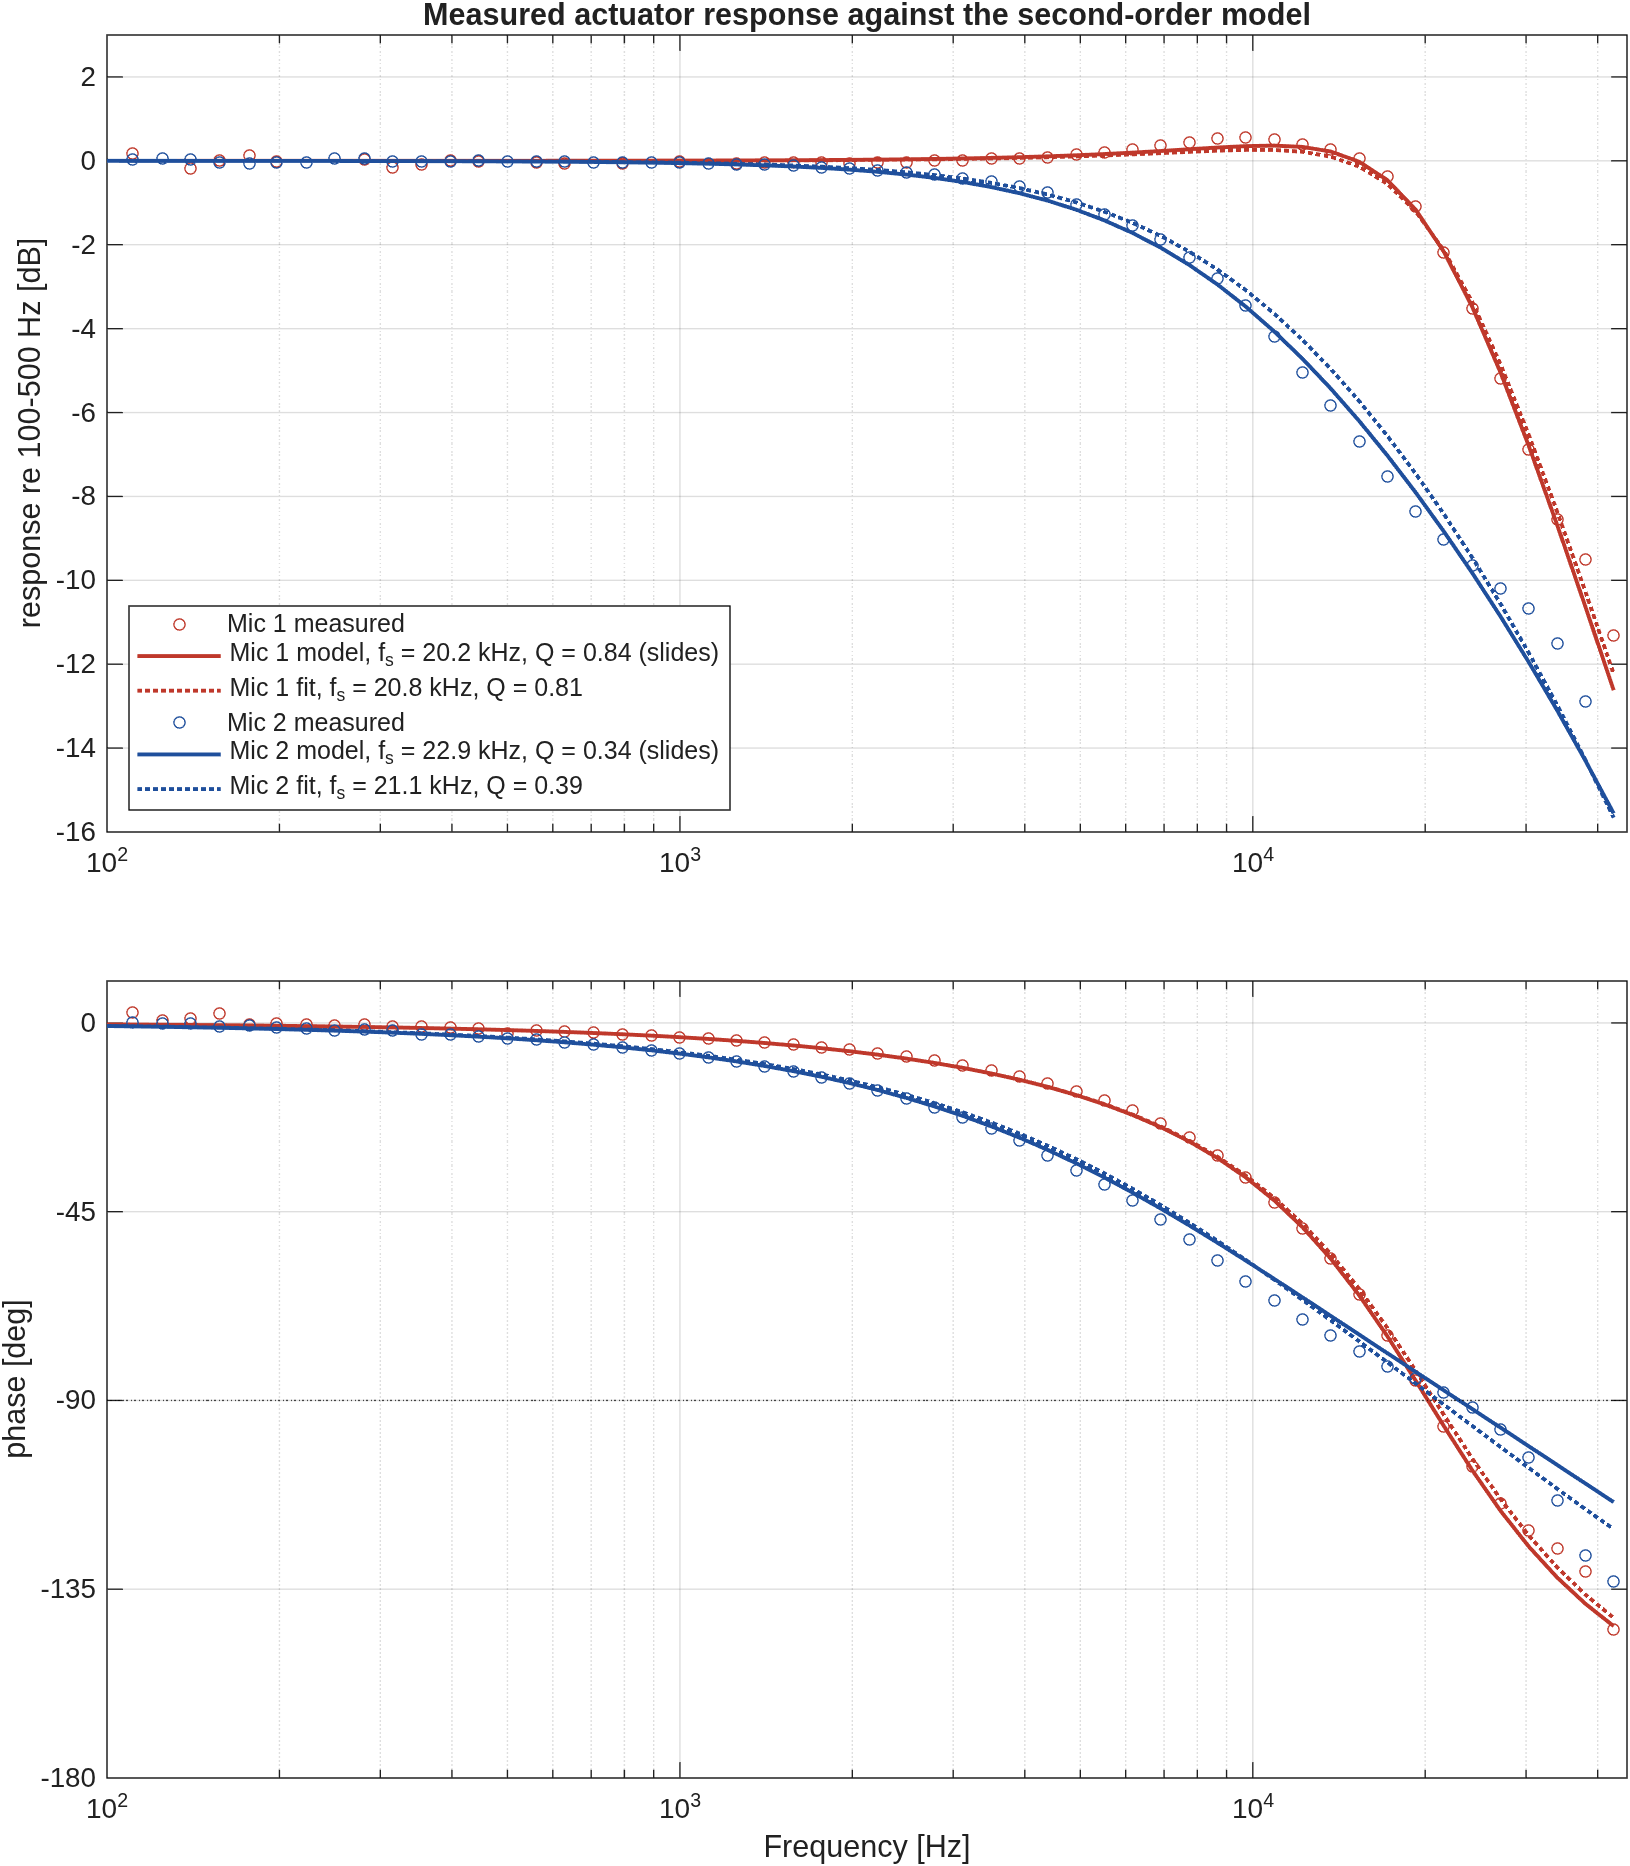
\includegraphics[width=0.85\linewidth]{labC_model_vs_measurement.png}
\caption{Shape only: measurement normalised to the \SI{100}{\hertz}--\SI{500}{\hertz}
level, with the model from the slide values (solid) and from the fit (dotted).}
\end{figure}

\begin{itemize}
\item \textbf{4134 (Mic 1):} the model follows the measurement within about
\SI{1.3}{\decibel} and \SI{8}{\degree} over the whole band, and within a few tenths of a
dB up to \SI{20}{\kilo\hertz}. The absolute level is only \SI{0.13}{\decibel} below the
calibration. The lumped model describes this capsule well without any adjustment.
\item \textbf{4133 (Mic 2):} most of the visible gap in the absolute plot is level, not
shape. The model's sensitivity is \SI{1.36}{\decibel} below the calibration, because it
uses one fixed $E C_{MT} S_D/x_0$ for both capsules while the real 4133 and 4134 differ in
compliance and gap (the brief's appendix). Aligned at \SI{1}{\kilo\hertz}, the shape
agrees within \SI{0.5}{\decibel} and \SI{5}{\degree} up to \SI{20}{\kilo\hertz}. Above
resonance the measurement departs by up to \SI{1.6}{\decibel} and \SI{19}{\degree}: the
phase falls slowly between about 12 and \SI{25}{\kilo\hertz} and then faster than the
model. One lumped $R_{AS}$ and $M_{AS}$ cannot follow the frequency-dependent air-film
damping of a free-field capsule everywhere, which is also why the slide reading and the
fit differ by 9\,\% in $f_s$.
\end{itemize}

\section{Conclusion}
\begin{itemize}
\item At \SI{1}{\kilo\hertz}, Mic 1 (B\&K 4134) has $M=\SI{10.98}{\milli\volt\per\pascal}$
(\SI{-39.2}{\decibel} re \SI{1}{\volt\per\pascal}) and Mic 2 (B\&K 4133) has
$M=\SI{13.03}{\milli\volt\per\pascal}$ (\SI{-37.7}{\decibel}). The expanded uncertainty
is about 2.8\,\% ($k=2$), dominated by the calibrator.
\item The three calibrators agree within 0.2\,\%, but the \SI{250}{\hertz} method reads
4\,\% low for both microphones. This is a systematic effect of the method, a clear example
of repeatability not implying accuracy.
\item The flat actuator response identifies Mic 1 as the pressure-field 4134
($f_s=\SI{20.2}{\kilo\hertz}$, $Q=0.84$). The strongly damped response identifies Mic 2
as the free-field 4133 ($f_s=\SI{22.9}{\kilo\hertz}$, $Q=0.34$).
\item The LTspice model with $M_{AS}$ and $R_{AS}$ from ($f_s$, $Q$) reproduces the 4134
closely. The 4133 is reproduced up to its resonance; above it the lumped model reaches
its limit, because the capsule's damping is not a single lumped element.
\item The actuator gives the shape of the pressure response quickly and with a large
signal-to-noise ratio, but not its absolute level and not the free-field response.
An acoustic calibration is still needed for the level, and a free-field correction for
use in a sound field.
\end{itemize}

\section*{Processing record}
\small
Raw data: \file{Lab C/raw data/} (lab-PC folder, unchanged: \file{datas_part1.mat},
\file{datas_part2.mat}, \file{datas_part3.mat}, \file{all.mat} and the scripts as run).
Processing: \file{Lab C/matlab/part1_system_reference.m} to \file{part4_model.m}
(\file{run_all.m}). Model: \file{Lab C/ltspice/gen_labC_ltspice.py --export --verify}
(LTspice agrees with the closed-form second-order model within $10^{-6}$). Brief: DTU
34870, \emph{Lab C -- Microphone calibration -- E26}.
\end{document}
